\section{Case Studies}


\subsection{Controlled Studies I - Autoregressive Process} \label{sec:ar-study}


In our simulation exercise the performance of QRAL model is evaluated by simulating data from an AR(1) model and then trying to recover its quantiles using QRAL and other competing models, namely:
\begin{enumerate}
\item \textbf{Quantile Regularized Adaptive LASSO (QRAL)}, which estimates a different model for each quantile $Q_{y_t|X}(\alpha,\cdot)$, for all ${j \in J}$. In practice, it means that each coefficient $\beta_{1j}$ is estimated with regularization on each quantile. %As the QRAL estimates a different solution for all every $\alpha$-quantile of $y_t$, the model $$y_t^{\alpha_j} = \beta_{0\alpha_j} + \beta_{\alpha_j} y_{t-1}, \quad \text{for all } j \in J$$ will produce as output a different model for each probability quantile $y_t^{\alpha_j}$.
\item \textbf{Quantile Regression as Koenker (QRK)} as originally proposed by \cite{koenker1978regression}, where each coefficient $\beta_{1j}$ is estimated independently using QR. 
\item A simple \textbf{Autoregressive (AR)} process.
\end{enumerate}

The AR(1) specification is given by:
\begin{equation}
y_t = \beta_0 + \beta_1 y_{t-1} + \varepsilon_t, \quad \varepsilon_t \sim N(0, 1), \quad t=1,\dots,400 \label{eq:ar1}
\end{equation}
with $\beta_0 = 0$, $\beta_1 = 0.3$ and $y_0 = 0$. This length is chosen due to the fact that the sample size of RG time series have such size in general.

The inter-quantile regularization parameter $\gamma$ (see Eq.(\ref{eq:adaLASSO-1})-(\ref{eq:adaLASSO-ult})) is estimated using cross-validation, a popular technique to select the best value of parameters for cross-sectional data. 
Since in this experiment the model has only one lag, model selection will not be evaluated, hence $\lambda=0$.
After simulating 1000 different time series given by Equation (\ref{eq:ar1}), the three models are estimated.
% TODO referência cross-validation

Since the main objective of this simulation experiment is to evaluate how our nonparametric model can correctly recover the true AR(1) process, model performance can be evaluated by examining how closely the estimated quantiles are from the populational ones. The results for each model are depicted in Figure \ref{fig:boxplot-ar1}, where a Boxplot containing the results for the 1000 simulations is shown. %a single boxplot for AR(1) and one for each probability $\alpha$ for QRAL and QRK.
\begin{figure}[ht]
	\centering
	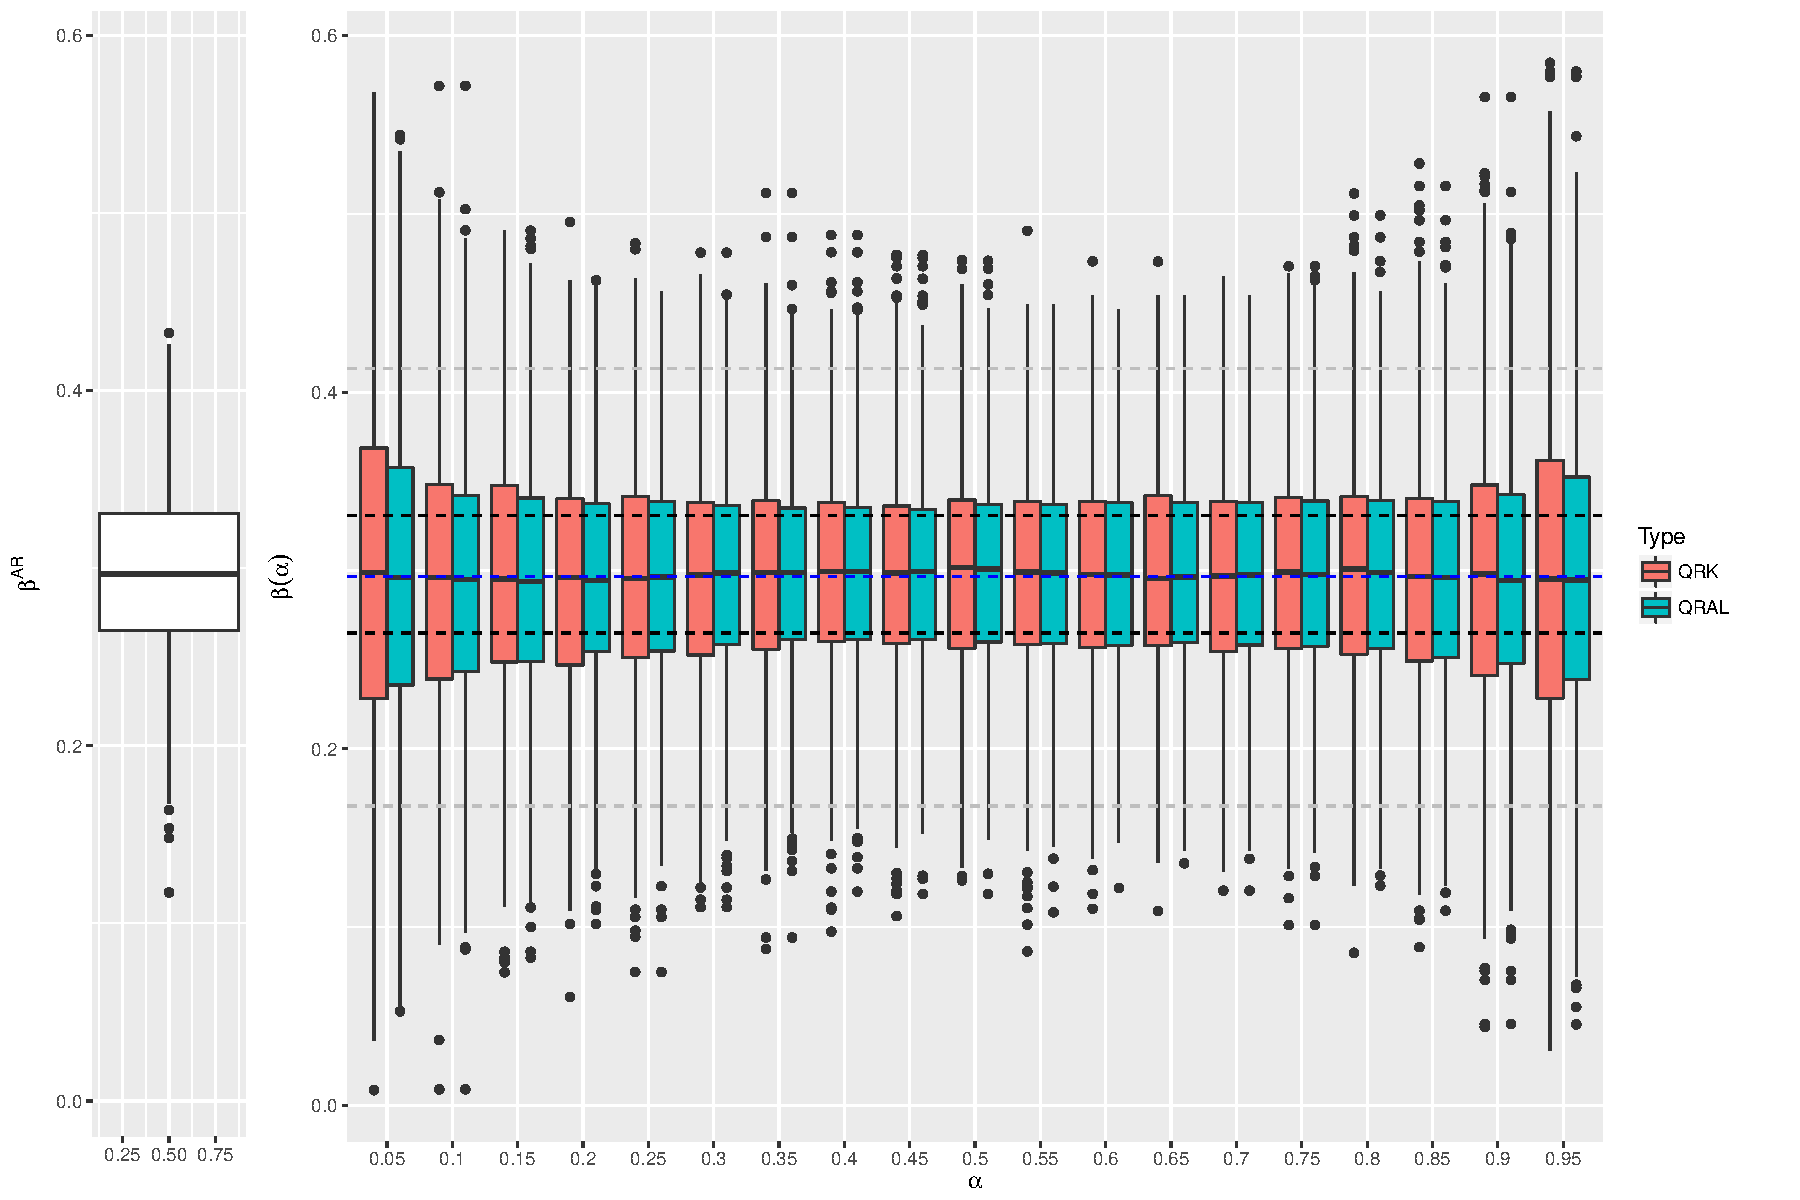
\includegraphics[width=1.0\linewidth]{Images/boxplot-ar1.pdf}
	\caption{Boxplot showing estimated coefficient after 1000 iterations. On the left hand side, the boxplot of the AR(1) coefficient estimation. Note that for the AR(1) the coefficient is equal for all probabilities $\alpha$. On the right hand side, the boxplot of the regular QR (where $\gamma = 0$) and the QRAL where $\gamma$ is selected using cross-validation. }
	\label{fig:boxplot-ar1}
\end{figure}
The conclusions from this experiment are: (i) coefficient estimation errors for the central quantiles are not far from those estimated by the AR model; (ii) extreme quantiles are usually harder to estimate, due to having fewer observations, and as a consequence, the estimation error increases on the extremes (iii) QRAL has an advantage over QRK by showing smaller variance of estimators.


\subsection{Case study with real data}

In this section, the QRAL methodology is tested in generating future scenarios for a real RG time series. The wind power time series, measured in megawatts, is composed of 31 years (from 1981 to 2011) of monthly observations from a wind farm located in the Brazilian Northeast. % Figure \ref{fig:icaraizinho-mensal} depicts a time series plot from which a strong seasonal pattern can be seen. 
The annual seasonality is seen in Figure \ref{fig:icaraizinho-mensal}, where each individual year is plotted as a single line on the graph. 
\begin{figure}[ht]
\centering
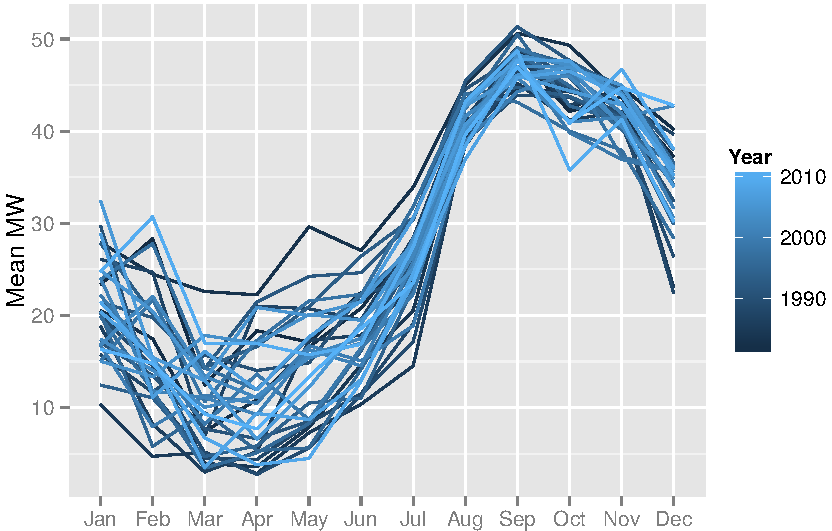
\includegraphics[width=0.8\linewidth]{Images/icaraizinho-mensal2.pdf}
\caption{Icaraizinho annual data. Each series consists of monthly observations for each year.}
\label{fig:icaraizinho-mensal}
\end{figure}

We use four different models to generate scenarios for monthly wind power time series:  QRAL, QRK, QRL (Quantile Regularized LASSO is essentially the same model as QRAL in which we let $w_{ij} = 1$, for all $i$ and $j$) and SARIMA. 
The tuning parameters $\lambda$ and $\gamma$ of QRL and QRAL are selected according to the two metrics presented on Section \ref{sec:estimation-evaluation-simulation}: SIC and GFS.

The estimated coefficients for the QR based models are presented in Figures \ref{fig:betas-qrk}-\ref{fig:betas-sic}. 
\begin{figure}[ht]
	\centering
	\includegraphics[width=1.0\linewidth]{Images/Betas-icaraizinho-QRK.pdf}
	\caption{Estimated coefficients for the QRK model.}
	\label{fig:betas-qrk}
\end{figure}
\begin{figure}[ht]
	\centering
	\includegraphics[width=1.0\linewidth]{Images/Betas-icaraizinho-GFS.pdf}
	\caption{Estimated coefficients for the QRAL (GFS) model.}
	\label{fig:betas-gfs}
\end{figure}
\begin{figure}[ht]
	\centering
	\includegraphics[width=1.0\linewidth]{Images/Betas-icaraizinho-SIC.pdf}
	\caption{Estimated coefficients for the QRAL (SIC) model.}
	\label{fig:betas-sic}
\end{figure}
We show for QRAL and QRK coefficients estimates for obtained via selection criteria. For each of these models, $\beta_0(\alpha)$ is shown on the left hand side figure, while $\beta(\alpha)$, for each lag, is on the right side.
The biggest difference between QRK and QRAL (via SIC) is that the former presents $\beta$ coefficients which are noisier and have higher variability between quantiles (as seen on experiment of section \ref{sec:ar-study}), given that, for this model, for each quantile $j$ a completely separated estimation problem is solved. Our proposed model has the advantage that quantiles are jointly estimated in a single model, which helps to decrease variance of estimators. Regularization of covariates plays a larger role in QRAL (via GFS criteria), where fewer covariates are left nonzero.

We also estimate a SARIMA model using the \emph{forecast} \cite{hyndman2008forecastpackage} package from R software, via the \emph{auto.arima} function, which selects the best model according to an IC (details on \cite{hyndman2008forecastmanual}). Even though the fully automatic estimation procedure did not select seasonal differencing, we force this operation in order to produce better scenarios according to the GFS metric. The best SARIMA model is $(2,0,2)\times(2,1,0)$ with drift and monthly seasonals.


The resulting tuning parameters estimates followed by SIC and GFS metric values for all models are shown on Table \ref{tab:results-icaraizinho}. When comparing the performance  of QRAL and QRL, we see that for either metric the adaptive LASSO produces a better estimation. 
QRAL, regularized via SIC, performs better than QRK for both metrics, but produces worse scenarios than SARIMA. There is a trade-off between having a good model for the short term (SIC metrics) and having a good model for producing scenarios on the long term (GFS metrics). 
When choosing the GFS metric, that has a better fit for generating scenarios, the chosen model must be able to select important features over the long term. On the other hand, when the model is tuned via SIC, more variables are selected and as a result the model is able to capture better short term fluctuations.
With selection by GFS, the size of the regularization parameters are bigger than those obtained via SIC, and the effect of larger parameters is seen clearly when comparing Figure \ref{fig:betas-gfs} with Figure \ref{fig:betas-sic}, as the coefficients shrinkage is much stronger on QRAL (GFS) than in QRAL (SIC). It is interesting to notice that the best QRAL model according to the metric GFS has fewer nonzero coefficients than that selected by optimizing SIC, but has the best results in minimizing the MAE with respect to the historic quantiles.  
\begin{table}[ht]
	\centering
	\caption{Cumulated statistics across all $\alpha_j$ quantiles}
	\label{tab:results-icaraizinho}
	\begin{tabular}{|l|c|c|c|c|}
		\hline 
		Method (tuning criteria) & $\lambda$ & $\gamma$ & SIC & GFS\tabularnewline
		\hline 
		\hline 
		QRL   (SIC) & 0.75 & 0.8 & 12.18 & 5.43\tabularnewline
		\hline 
		QRAL   (SIC) & 0.25 & 0.8 & 12.15 & 5.41\tabularnewline
		\hline 
		QRL    (GFS) & 9.02 & 33.1 & 13.68 & 4.58\tabularnewline
		\hline 
		QRAL   (GFS) & 1.82 & 90.01 & 13.63 & 4.23\tabularnewline
		\hline 
		QRK    ( - ) & 0 & 0 & 13.00 & 5.92 \tabularnewline
		\hline 
		SARIMA ( - ) & - & - & - & 5.15 \tabularnewline
		\hline 	
	\end{tabular}
	\end{table}
	

% The accuracy of the generated scenarios - considering the MAE metric - in recovering the historic quantiles for each month is the metric used for evaluation.

% In Figure \ref{fig:simulated-quantiles}, we compare three specific quantiles (5\%, 50\% and 95\%) of the historic data with SARIMA and QRAL (with tuning by GFS) over the 12 months of the third simulated year, as explained on the section  \ref{sec:GFS} about GFS. 
% \begin{figure}[h]
% 	\centering
% 	\includegraphics[width=1.0\linewidth]{Images/Comparison-scenarios-icaraizinho.pdf}
% 	\caption{Estimated quantiles 5\%, 50\% and 95\% of SARIMA and QRAL in comparison with historic quantiles.}
% 	\label{fig:simulated-quantiles}
% \end{figure}
In Figures \ref{fig:scenarios-qral} and \ref{fig:scenarios-sarima}, we compare the median (50\%), extreme quantiles (5\% and 95\%) and the 1st and 3rd quartiles (25\% and 75\%) obtained from  both QRAL and SARIMA models via simulation, with the associated historical quantiles. The period of simulation is the same employed for the metric GFS, that is for the year 2014. As it can be seen, the results from QRAL are better in capturing the unconditional seasonality than those produced by SARIMA, as the former's quantiles are closer to the historic quantiles than the latter's.


% \begin{figure}[h]
% 	\centering
% 	\includegraphics[width=1.0\linewidth]{Images/QRAL-historic-icaraizinho}
% 	\caption{Historic quantiles of icaraizinho}
% 	\label{fig:betas-gfs}
% \end{figure}
\begin{figure}[ht]
	\centering
	\includegraphics[width=1.0\linewidth]{Images/ScenariosHHH3-QRAL-icaraizinho.pdf}
	\caption{Comparison of unconditional generated scenarios (the third year of simulation) with historic quantiles of QRAL.  The areas represent QRAL quantiles ($5\%-95\%$),
	while the historic quantiles are marked by symbols, by month. }
	\label{fig:scenarios-qral}
\end{figure}

\begin{figure}[h]
	\centering
	\includegraphics[width=1.0\linewidth]{Images/ScenariosHHH3-SARIMA-icaraizinho.pdf}
	\caption{Comparison of unconditional generated scenarios (the third year of simulation) with historic quantiles of SARIMA. The areas represent SARIMA quantiles ($5\%-95\%$),
	while the historic quantiles are marked by symbols, by month. }
	\label{fig:scenarios-sarima}
\end{figure}
